\chapter{Inverse}

\section{Left Inverse, Right Inverse, Inverse}

\begin{definition}[$A$的左逆]
    当一个矩阵X满足 $$ X A=I $$ 
    
    X被称为 $ A $ 的\textit{左逆}; 当左逆存在时,则称A是\textit{可左逆}的;
\end{definition}

    如果左逆矩阵存在, 则左逆矩阵有\textbf{无穷多}个.

\begin{example}
    $$ A=\left[\begin{array}{cc}-3 & -4 \\ 4 & 6 \\ 1 & 1\end{array}\right] $$

    矩阵$A$是可左逆的,其左逆矩阵有两个

    $$ B=\frac{1}{9}\left[\begin{array}{ccc}-11 & -10 & 16 \\ 7 & 8 & -11\end{array}\right] \quad C=\frac{1}{2}\left[\begin{array}{ccc}0 & -1 & 6 \\ 0 & 1 & -4\end{array}\right] $$
\end{example}

\begin{definition}[$A$的右逆]
    当左逆存在时,则称A是可左逆的;
\end{definition}

    如果右逆矩阵存在, 则右逆矩阵有\textbf{无穷多}个.


\begin{example}
    $$ B=\left[\begin{array}{lll}1 & 0 & 1 \\ 0 & 1 & 1\end{array}\right] $$

    矩阵$B$可右逆,以下矩阵都是$B$的右逆

    $$ D=\frac{1}{2}\left[\begin{array}{cc}1 & -1 \\ -1 & 1 \\ 1 & 1\end{array}\right], E=\left[\begin{array}{ll}1 & 0 \\ 0 & 1 \\ 0 & 0\end{array}\right], G=\left[\begin{array}{cc}1 & -1 \\ 0 & 0 \\ 0 & 1\end{array}\right] $$
\end{example}

一个大小为 $ m \times n $ 的矩阵, 其左逆或右逆的维度为 $ n \times m $.

\begin{theorem}
    A的左逆为 $ X $ 当且仅当 $ X^{T} $ 是 $ A^{T} $ 的右逆.
\end{theorem}

\begin{proof}
    $$
A^{T} X^{T}=(X A)^{T}=I
$$
\end{proof}

\begin{theorem}
    A的右逆为 $ X $ 当且仅当 $ X^{T} $ 是 $ A^{T} $ 的左逆.
\end{theorem}

\begin{proof}
    $$
X^{T} A^{T}=(A X)^{\mathrm{T}}=I
$$
\end{proof}

\begin{theorem}
    如果矩阵A存在左逆和右逆,则左逆和右逆一定相等
\end{theorem}

\begin{proof}
    $$
    \begin{aligned}
    &X A=I, A Y=I  \\
    \Rightarrow&  X=X I=X(A Y)=(X A) Y=Y \\
    \Rightarrow& X=Y
    \end{aligned}
$$
\end{proof}

\begin{definition}
    如果矩阵A存在左逆和右逆, 此时X称为矩阵的\textit{逆},记作 $ A^{-1} $ 当矩阵的逆存在时,则称矩阵A\textit{可逆}.
\end{definition}

\section{Linear Equation Systems}

\begin{definition}
    有$n$个变量的$m$个方程为

    $$ \left\{\begin{array}{c}A_{11} x_{1}+A_{12} x_{2}+\cdots+A_{1 n} x_{n}=b_{1} \\ A_{21} x_{1}+A_{22} x_{2}+\cdots+A_{2 n} x_{n}=b_{2} \\ \vdots \\ A_{m 1} x_{1}+A_{m 2} x_{2}+\cdots+A_{m n} x_{n}=b_{m}\end{array}\right. $$

    写成矩阵形式为: $ \mathrm{A} x=\mathrm{b} $ . 其中$A$为系数矩阵, $ x $ 为$n$维列向量. 
\end{definition}

该方程组可能\textbf{无解},\textbf{有唯一解}和\textbf{无穷解}.

\subsection{线性方程组求解}

\begin{theorem}
    如果矩阵$A$可左逆,假设 $ X $ 是矩阵$A$的左逆,则\textbf{至多}一个解, 如有解则 $ x=X b $ 。
\end{theorem}

\begin{proof}
    $$
A x=b \Rightarrow  x=X A x=X b
$$
\end{proof}

\begin{theorem}
    如果矩阵$A$可右逆,假设 $ Y $ 是矩阵$A$的右逆,则\textbf{至少}一个解, 即 $ x=\mathrm{Y} b $ 。
\end{theorem}

\begin{proof}
    设$x=Y b$ 

    $$
x=Y b  \Rightarrow  A x=A Y b=b
$$
\end{proof}

\begin{theorem}
    如果矩阵$A$可逆的,假设 $ X $ 是矩阵$A$的逆,则
$$
A x=b  \Rightarrow  x=A^{-1} b
$$
唯一解。
\end{theorem}

\section{非奇异矩阵}

\begin{theorem}
    对于方阵 $ A \in \mathbb{R}^{n \times n} $ ,以下条件都是等价的:

    \begin{enumerate}
        \item $ A $ 可左逆
        \item $A$的列向量线性无关
        \item $A$可右逆
        \item $A$的行向量线性无关
        \item $A$可逆
    \end{enumerate}

    此时矩阵$A$为非奇异矩阵,由条件1与3,可得$A$为可逆矩阵。
\end{theorem}

\begin{proof}
    可以通过以下方式证明:

    \centering
    \tikzset{every picture/.style={line width=0.75pt}} %set default line width to 0.75pt        

    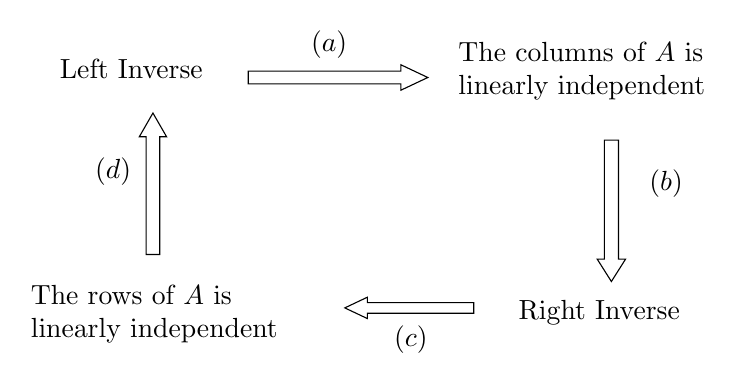
\begin{tikzpicture}[x=0.75pt,y=0.75pt,yscale=-1,xscale=1]
    %uncomment if require: \path (0,300); %set diagram left start at 0, and has height of 300

    %Right Arrow [id:dp1873650424277289] 
    \draw   (269,87.07) -- (342.52,87.07) -- (342.52,84) -- (355.52,90.14) -- (342.52,96.27) -- (342.52,93.2) -- (269,93.2) -- cycle ;
    %Right Arrow [id:dp6482140902579632] 
    \draw   (219.8,175.44) -- (219.8,118.66) -- (216.53,118.66) -- (223.08,107.27) -- (229.64,118.66) -- (226.36,118.66) -- (226.36,175.44) -- cycle ;
    %Right Arrow [id:dp31978358236465754] 
    \draw   (447.37,120.34) -- (447.37,177.66) -- (450.78,177.66) -- (443.96,188.43) -- (437.14,177.66) -- (440.55,177.66) -- (440.55,120.34) -- cycle ;
    %Right Arrow [id:dp9972986143574651] 
    \draw   (377.64,198.57) -- (326.37,198.57) -- (326.37,196) -- (315.52,201.14) -- (326.37,206.27) -- (326.37,203.7) -- (377.64,203.7) -- cycle ;

    % Text Node
    \draw (177,80) node [anchor=north west][inner sep=0.75pt]   [align=left] {Left Inverse};
    % Text Node
    \draw (369,72) node [anchor=north west][inner sep=0.75pt]   [align=left] {The columns of $A$ is\\ linearly independent};
    % Text Node
    \draw (163,189) node [anchor=north west][inner sep=0.75pt]   [align=left] {The rows of $A$ is\\ linearly independent};
    % Text Node
    \draw (398,196) node [anchor=north west][inner sep=0.75pt]   [align=left] {Right Inverse};
    % Text Node
    \draw (298,66.4) node [anchor=north west][inner sep=0.75pt]    {$( a)$};
    % Text Node
    \draw (338,208.4) node [anchor=north west][inner sep=0.75pt]    {$( c)$};
    % Text Node
    \draw (461,133.4) node [anchor=north west][inner sep=0.75pt]    {$( b)$};
    % Text Node
    \draw (194,127.4) node [anchor=north west][inner sep=0.75pt]    {$( d)$};


    \end{tikzpicture}

    \begin{itemize}
        \item 性质 $ (\mathrm{a}) $ 对任意矩阵 $ A \in \mathbb{R}^{m \times n} $ 都成立 
        \item 性质$(b)$对方阵矩阵 $ A \in \mathbb{R}^{n \times n} $ 都成立
        \item 对于性质 $ (\mathrm{c}) $ 与 $ (\mathrm{d}) $, 可利用 $ A^{T} $ 证明
    \end{itemize}
\end{proof}

\begin{theorem}
    $(a)$: $A$可左逆,则$A$列向量线性无关.
\end{theorem}

\begin{proof}
    假设$A$的左逆是 $ B $ ,则
    $$
    \begin{aligned}
            & A x=0 
     \Rightarrow &B A x=0 \\
    \Rightarrow & I x=0
    \end{aligned}
    $$

    假设A的列向量 $ A=\left[a_{1}, a_{2}, \cdots, a_{n}\right] $
    $$
    A x=x_{1} a_{1}+x_{2} a_{2}+\cdots+x_{n} a_{n}=0
    $$

    则当该等式 $ A x=0 $ 成立时,其解 $ x=0 $, 则A的列向量线性无关。 
    
    \begin{corollary}
        如果 $ A \in \mathbb{R}^{m \times n} $有左逆,则有 $ m \geq n  $。

    即$A$是高或方的矩阵, 如 $ A=\left[\begin{array}{ll}1 & 0 \\ 0 & 1 \\ 0 & 0\end{array}\right] $.
    \end{corollary}
    

    假设 $ A $ 的列向量 $ A=\left[a_{1}, a_{2}, \cdots, a_{n}\right] $
    $$
    \begin{aligned}
         A x&=x_{1} a_{1}+x_{2} a_{2}+\cdots+x_{n} a_{n}=b \\
    A y&=y_{1} a_{1}+y_{2} a_{2}+\cdots+y_{n} a_{n}=b \\
    \end{aligned}
    $$

    $$A x-A y=A(x-y)=0 \Rightarrow x=y$$

    当 $ b \in \mathbb{R}^{m}, b \notin\left\{y \mid y=A x, x \in \mathbb{R}^{n}\right\} $ 时(即$b$不在$A$的列空间,$ m \geq n  $时),线性方程组无解。 $ A x=b $ 至多一个解,如有解则 $ x=X b $ 。
\end{proof}

\begin{theorem}
    矩阵的行秩等于列秩.
\end{theorem}

\begin{proof}
    令 $A$ 是一个 $m\times n$ 的矩阵,其列秩为 $r $. 因此矩阵 $A$ 的列空间的维度是 $r$ . 
    
    令 $c_1,c_2,\ldots,c_r$ 是 $A$ 的列空间的一组基,构成 $m \times r$ 矩阵 $C$ 的列向量 $C = [c_1,c_2,\ldots,c_r]$,并使得 $A$ 的每个列向量是 $C$ 的 $r$ 个列向量的线性组合. 
    
    由矩阵乘法的定义,存在一个 $r \times n$ 矩阵 $R$, 使得 $A = CR$. ($A$ 的 $(i,j)$ 元素是 $c_i$ 与 $R$ 的第 $j$ 个行向量的点积.)

现在,由于 $A = CR$, $A$ 的每个行向量是 $R$ 的行向量的线性组合,这意味着 $A$ 的行向量空间被包含于 $R$ 的行向量空间之中. 因此 $A 的行秩 \leq R的行秩$. 但R仅有$r$行, 所以$R的行秩 \leq r = A的列秩$. 这就证明了$A的行秩 \leq A的列秩$.

把上述证明过程中的“行”与“列”交换,利用对偶性质同样可证$A的列秩 \leq A的行秩$。更简单的方法是考虑A的转置矩阵 $A^\mathrm{T}$,则$A的列秩 =  A^\mathrm{T}的行秩 \leq  A^\mathrm{T}的列秩 = A的行秩$. 这证明了$A$的列秩等于$A$的行秩. 证毕.
\end{proof}

\begin{theorem}
    $(c)$: 矩阵 $ A \in \mathbb{R}^{m \times n} $ 有右逆 $ X $, 则A行向量线性无关.
\end{theorem}

\begin{proof}
    $$ \mathrm{X}^{T} A^{T}=(A X)^{T}=I $$
    
    则有 $ \mathrm{X}^{T} $ 是 $ A^{T} $ 的左逆, $ A^{T} $ 的列向量线性无关。 

    即 $ A^{T} \in \mathbb{R}^{n \times m} $.
    
    \begin{corollary}
     如果 $ A \in \mathbb{R}^{m \times n} $有左逆,则有 $ m \leq n  $。

    即$A$是宽或方的矩阵.   
    \end{corollary}
    
    根据定理“矩阵的行秩等于列秩”,$ A^{T} $ 的列向量线性无关,则矩阵 $ A $ 有$m$个线性无关列向量(行向量),即通过 Gram-Schmidt 正交化可得$m$个正交基。

    $ \forall b \in \mathbb{R}^{m} $, 有 $ b \in\left\{y \mid y=A x, x \in \mathbb{R}^{n}\right\} (m \leq n ) $, 方程 $ A x=b $ 有解,其解为 $ x=X b $ 。
\end{proof}

\begin{theorem}
    $(b)$: 若方阵A列向量线性无关,则A可右逆。
\end{theorem}

\begin{proof}
    假设 $ A \in \mathbb{R}^{n \times n} $ 为方阵且列向量线性无关 
    
    $$ A=\left[a_{1}, a_{2}, \cdots, a_{n}\right] $$

    则对于任意向量 $ \mathrm{b} \in \mathbb{R}^{n} $, 则向量组 $ \left[a_{1}, a_{2}, \ldots, a_{n}, \mathrm{~b}\right] $ 线性相关,存 在不全为0的系数,使得以下等式成立
    $$
    x_{1} a_{1}+x_{2} a_{2}+\cdots+x_{n} a_{n}+x_{n+1} b=0
    $$

    因为$A$列向量线性无关,则 $ x_{n+1} \neq 0 $(假设$ x_{n+1} = 0 $会推出违反线性无关假设的结论), 即$b$是$A$列向量的线性组合;
    $$
    b=-\frac{x_{1}}{x_{n+1}} a_{1}-\frac{x_{2}}{x_{n+1}} a_{2}-\cdots-\frac{x_{n}}{x_{n+1}} a_{n}
    $$

    存在向量 $ c_{1}, \ldots, c_{n} \in \mathbb{R}^{n} $,使得 
    $$
    \begin{aligned}
        Ac _{1}&=e_{1}\\
         A c_{2}&=e_{2}\\
          \ldots \\
          A c_{n}&=e_{n}
    \end{aligned}
    $$

    则矩阵 $ C=\left[c_{1} c_{2} \ldots c_{n}\right] $ 是矩阵 $ A $ 的右逆, $ A C=I $.

\end{proof}

